\documentclass[a4paper]{article}

\usepackage[pdftex]{graphicx}
\usepackage[margin=3cm]{geometry}
\usepackage{verbatim,moreverb,amssymb,amsmath}


\newcounter{question}
\newcommand{\question}{\refstepcounter{question}\section*{Question~\thequestion}}
\renewcommand*\thequestion{\arabic{question}}


\begin{document}

\pagestyle{empty}
\thispagestyle{empty}



\noindent
\begin{minipage}{\columnwidth}
  \centering
  \Large
  DA4002 (HT11) Halmstad University\\
  Introduction to Algorithms, Data Structures, and Problem Solving\\[3\baselineskip]
  \Huge
  Written Exam\\
  \Large
  Monday, January 2, 2012\\[2\baselineskip]
  Examiner: Roland Philippsen
\end{minipage}

\vfill

\noindent
\begin{center}
\fbox{
  \begin{minipage}{0.8\columnwidth}
    \textbf{Student Name:}\\[3\baselineskip]
  \end{minipage}
}
\end{center}

\vfill



\section*{Rules}

Aside from the obvious rules of conduct exams (e.g.\ no chatting):

\begin{itemize}
\item
  \textbf{No computing devices} (laptops, phones, calculators, \emph{etc}).
\item
  \textbf{No books or printouts}.
\item
  \textbf{Allowed self-written notes}: two sheets of A4 paper (front and back).
\end{itemize}



\section*{General Guidelines}

\begin{itemize}
\item
  \textbf{Read carefully} and pace yourself.
  You can solve the problems in any order you want, but later problems may be easier to solve after you have answered the preceding questions.
\item
  \textbf{Write clearly} and draw clear diagrams.
  If you need to correct a mistake, then cleanly cross out the wrong answer and clearly indicate where the correction can be found.
\item
  \textbf{Indicate the question number} for each of your answers.
  If a question has sub-questions, indicate the sub-question number after the main question number, separated by a dot.
  For example, question 3 has 4 sub-questions, and their answers should be numbered 3.1, 3.2, 3.3, and 3.4.
\end{itemize}



\pagebreak
\pagestyle{plain}
\thispagestyle{plain}
\setcounter{page}{1}



\question

For each of the following data storage examples, choose the most appropriate data structure types from the ones listed in the box.
Also, briefly explain your choice in writing, and draw a diagram to illustrate the chosen data structure.

\begin{center}
  \fbox{%
    \begin{minipage}{0.7\columnwidth}
      List of data structures to choose from:
      \begin{itemize}
      \item linked list
      \item undirected graph
      \item directed graph
      \item k-ary tree
      \item binary search tree
      \end{itemize}
    \end{minipage}%
  }
\end{center}


\begin{enumerate}
\item
  Storing a log (time series) of meteorological data containing temperature, atmospheric pressure, wind speed, and wind direction.
  The purpose of the log is to later display graphs of the evolution over time of these data.
\item
  Keeping an inventory of electronical components in a workshop, such as various resistors, capacitors, transistors, etc.
  The purpose is to look up components by part number to see how many are in stock.
\item
  Tracking the prerequisite dependencies between courses at a University.
  The purpose is to help students plan their curriculum and allow professors to check for inconsistencies in study programmes.
\item
  Storing information about animals and plants that are on display in a museum of natural history.
  The purpose is to present visitors with an interface where they can explore the collection according to biological classification.
  For example, animal are grouped into species, which are parts of a genus, which are grouped into families.
\end{enumerate}

\clearpage

\question

For each of the following code fragments,
\begin{itemize}
\item
  develop a formula allowing to estimate the running time depending on the parameter $N$,
\item
  and then determine its Big-Oh runtime complexity.
\end{itemize}

\noindent
Note that the method \texttt{f\_1ms} requires 1 ms to run, and the method \texttt{f\_3ms} needs 3 ms.
All other operation delays can be neglected.

\begin{itemize}
\item
  fragment 1:\\
  \begin{minipage}[t]{0.4\columnwidth}
    \footnotesize
    \verbatimtabinput{q2a.txt}
  \end{minipage}
\item
  fragment 2:\\
  \begin{minipage}[t]{0.4\columnwidth}
    \footnotesize
    \verbatimtabinput{q2b.txt}
  \end{minipage}
\item
  fragment 3:\\
  \begin{minipage}[t]{0.4\columnwidth}
    \footnotesize
    \verbatimtabinput{q2c.txt}
  \end{minipage}
\item
  fragment 4:\\
  \begin{minipage}[t]{0.4\columnwidth}
    \footnotesize
    \verbatimtabinput{q2d.txt}
  \end{minipage}
\end{itemize}

\clearpage

\question

The following four diagrams define the directed graphs \textbf{G1}, \textbf{G2}, \textbf{G3}, and \textbf{G4}.\\[1.2\baselineskip]
\centerline{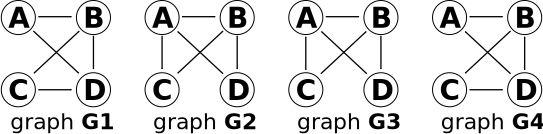
\includegraphics[width=0.6\columnwidth]{q3-graphs.pdf}}\\[1.2\baselineskip]
\noindent
There are many ways of defining and storing such graphs, for example the three possibilities labeled \textbf{D1}, \textbf{D2}, and \textbf{D3} in the three boxes below:\\

\noindent
\fbox{%
  \begin{minipage}[t]{0.3\columnwidth}
    definition \textbf{D1}\\
    \emph{adjacency lists}\\[1.1\baselineskip]
    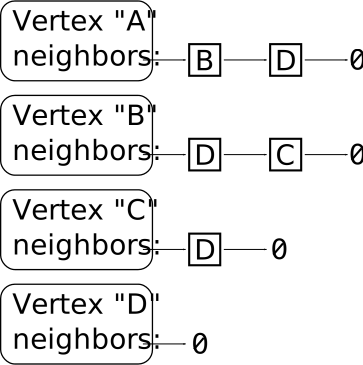
\includegraphics[width=\columnwidth]{q3-adjlist-diagrams.pdf}
  \end{minipage}%
}
\hfill
\fbox{%
  \begin{minipage}[t]{0.3\columnwidth}
    definition \textbf{D2}\\
    \emph{source code}
    \footnotesize
    \verbatimtabinput{Q3.java}
  \end{minipage}%
}
\hfill
\fbox{%
  \begin{minipage}[t]{0.3\columnwidth}
    definition \textbf{D3}\\
    \emph{adjacency matrix}\\[1.1\baselineskip]
    \begin{tabular}{|*{5}{c|}}
      \hline
      \emph{source}
      &
      \multicolumn{4}{l|}{\emph{destination}} \\
        & A & B & C & D \\
      \hline
      A &   & * &   &   \\
      \hline
      B &   &   & * &   \\
      \hline
      C &   &   &   & * \\
      \hline
      D & * & * &   &   \\
      \hline
    \end{tabular}
  \end{minipage}%
}\\

\begin{enumerate}
\item
  For each of the definitions \textbf{D1}, \textbf{D2}, and \textbf{D3}, find out which of the graphs \textbf{G1}, \textbf{G2}, \textbf{G3}, and \textbf{G4} is created or represented.
\item
  One of the graphs is not represented by any of the definitions.
  Which one is it?
  Choose one of the definition styles and use that to describe the graph that was not covered by \textbf{D1}, \textbf{D2}, and \textbf{D3}.
\end{enumerate}

\clearpage

\question

A \emph{spanning tree} is a tree which is embedded in a graph in such a way that
(1) all the vertices of the graph appear in the tree, and
(2) all the edges of the tree are also edges in the graph.
In other words, a spanning tree is composed of all the vertices and some of the edges of the graph.
It is possible to compute a spanning tree by tracing the execution of depth-first search (DFS):
whenever a non-visited vertex is encountered, the edge connecting to it is added to the spanning tree.
This technique also works with breadth-first search (BFS), usually giving a different result.

\emph{%
For example, assume that you are in the middle of DFS and the current vertex is \textbf{V}.
Its neighbor \textbf{W} has not yet been visited, so the edge \textbf{(V,W)} is marked as belonging to the spanning tree before proceeding with the ongoing DFS.}

\begin{center}
  \fbox{%
    \begin{minipage}{0.95\columnwidth}
      \begin{minipage}{0.4\columnwidth}
        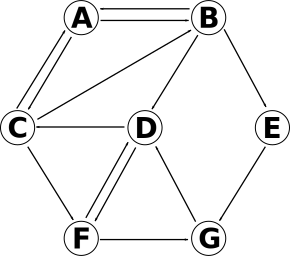
\includegraphics[width=\columnwidth]{q4-graph-diagram.pdf}
      \end{minipage}
      \hfill
      \begin{minipage}{0.45\columnwidth}
        \begin{tabular}{|*{8}{c|}}
          \hline
          \emph{source}
          &
          \multicolumn{7}{l|}{\emph{destination}} \\
            & A & B & C & D & E & F & G \\
          \hline
          A &   & * & * &   &   &   &   \\
          \hline
          B & * &   &   & * & * &   &   \\
          \hline
          C & * & * &   &   &   & * &   \\
          \hline
          D &   &   & * &   &   & * &   \\
          \hline
          E &   &   &   &   &   &   & * \\
          \hline
          F &   &   &   & * &   &   & * \\
          \hline
          G &   &   &   & * &   &   &   \\
          \hline
        \end{tabular}
      \end{minipage}
    \end{minipage}%
  }
\end{center}

The above diagram shows a directed graph.
Its adjacency matrix representation is also given, to define an iteration order for the edges.
This is important because it determines the vertex visitation order for the following questions.
The order is given by reading from left to right along the appropriate row of the adjacency matrix.
\emph{For example, the order of edges emanating from vertex \textbf{C} is: \textbf{A}, \textbf{B}, \textbf{F}.}

\begin{enumerate}
\item
  Perform DFS starting at vertex \textbf{D}.
  Write down the order in which the vertices are visited.
\item
  Perform BFS, also starting at vertex \textbf{D}, and also writing down the visitation order.
\item
  Draw a diagram of the spanning tree rooted at \textbf{A} using depth-first search.
\item
  Draw a diagram of the spanning tree rooted at \textbf{A} using breadth-first search.
\end{enumerate}

\clearpage

\question

Imagine that you have been hired by a company to help them with software development.
You are asked to fix the following broken code fragments:\\[1.2\baselineskip]

\noindent
\begin{minipage}{0.45\columnwidth}
  \fbox{%
    \begin{minipage}{\columnwidth}
      \footnotesize
      \verbatimtabinput{q5a.txt}
  \end{minipage}}\\[1.2\baselineskip]
  \fbox{%
    \begin{minipage}{\columnwidth}
      \footnotesize
      \verbatimtabinput{q5b.txt}
  \end{minipage}}
\end{minipage}
\hfill
\fbox{%
  \begin{minipage}{0.45\columnwidth}
    \footnotesize
    \verbatimtabinput{q5c.txt}
\end{minipage}}

\begin{enumerate}
\item
  An intern is trying to compute the Fibonacci sequence using dynamic programming.
  But the output of his method \texttt{fibonacci} is ``1, 1, 2, 4, 8, 16, 32, \ldots'' instead of ``1, 1, 2, 3, 5, 8, 13, \ldots''
  What is the problem?
  How can it be fixed?
\item
  An analyst is trying to speed up lookups on sorted data by using binary search instead of linear search.
  However, when given the test data ``\texttt{\{ 1, 23, 25, 66, 102 \}}'' his \texttt{binsearch} method fails to find the number 66, although it does find the number 25.
  What is the problem?
  How can it be fixed?
\item
  A call center technician is trying to use a linked list to manage queues of incoming phone calls.
  His implementation of the \texttt{Queue} class has a method \texttt{enqueue} to add items to the waiting list, and \texttt{dequeue} to remove the oldest item from the list.
  However, the \texttt{dequeue} method always returns \texttt{null} after it has returned one item, no matter how many items have been added using \texttt{enqueue}.
  What is the problem?
  How can it be fixed?
\end{enumerate}

\end{document}
